\section{Methodology}

\subsection{Study Area and Data}

All inputs are public data; none are synthesised for the optimisation
instance. Parcels are OpenStreetMap land-use polygons~\cite{osm}. Of 941
polygons, 625 have centroids outside the West Bank. The remaining 316 are
assigned to Oslo areas~\cite{ocha} by centroid and filtered to 0.1--100~ha,
leaving 174 parcels (1{,}464~ha) in Areas A/B and 110 (706~ha) in Area C
(Fig.~\ref{fig:map}). The Oslo layer merges Areas A and B into a single class.

\begin{figure}[t]
\centering
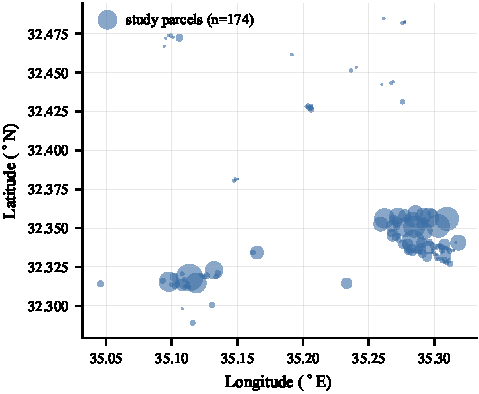
\includegraphics[width=0.92\columnwidth]{figures/fig_map.pdf}
\caption{Study parcels by Oslo area; marker area is proportional to parcel
size.}
\label{fig:map}
\end{figure}

Climate is NASA POWER~\cite{nasapower} for 2015--2024: 465~mm rainfall per
year (90\% in November--March), 20.7$^\circ$C and 68.7\% relative humidity.
NASA POWER resolves Jenin as one grid cell, so climate is identical across
parcels. Soil properties are SoilGrids 250\,m estimates~\cite{poggio2021},
available for 149 of the 174 A/B parcels (the rest take the governorate mean).

Producer prices are FAOSTAT~\cite{faostat} means for 2019--2023. We exclude
2024, when perishable prices rose 1.24--5.76$\times$ over 2023 while wheat
(0.95$\times$) and olives (1.10$\times$) did not, consistent with a wartime
supply shock rather than demand. Yields are FAOSTAT means for 2014--2022.
Because national vegetable yields include greenhouses, vegetables are rescaled
so their mean matches the PCBS open-field level for the northern West
Bank~\cite{pcbs} (19.65~t/ha), and tree crops so that olives match PCBS
(1.43~t/ha). Net irrigation requirements are indicative values following
FAO-56~\cite{allen1998}. Table~\ref{tab:crops} lists the resulting parameters.

\begin{table}[t]
\centering
\caption{Crop parameters}
\label{tab:crops}
\footnotesize
\begin{tabular}{lrrrr}
\toprule
Crop & Yield (t/ha) & Price (\$/t) & Water (m$^3$/ha) & Cost share \\
\midrule
wheat     &  2.41 &  568 &  500 & 0.65 \\
potatoes  & 13.27 &  488 & 4000 & 0.55 \\
tomatoes  & 51.74 &  628 & 6000 & 0.55 \\
cucumbers & 18.49 &  614 & 4500 & 0.55 \\
onions    &  9.56 &  526 & 3500 & 0.55 \\
eggplants & 19.04 &  459 & 6000 & 0.55 \\
maize     &  5.79 &  572 & 5000 & 0.65 \\
olives    &  1.43 & 1752 & 1500 & 0.40 \\
grapes    &  9.38 &  987 & 3000 & 0.40 \\
oranges   & 19.38 &  601 & 7000 & 0.40 \\
\bottomrule
\end{tabular}
\end{table}

Production cost is an assumption: a share of baseline gross revenue typical
of the system type, held fixed when prices are perturbed.

\subsection{Suitability Model}

A Random Forest (300 trees)~\cite{breiman2001} is trained on a public dataset
of 2{,}200 labelled observations over 22 crops~\cite{kagglecrop} with features
$(N,P,K,T,H,\mathrm{pH},R)$. Seven study crops are absent from it; labelled
rows for these are generated from FAO EcoCrop envelopes~\cite{ecocrop}. Real
and synthetic rows are evaluated separately. Suitability is
\begin{equation}
s_{ij}=\mathrm{RF}_j(\mathbf{x}_i)\,\phi(\ell_i,j),
\end{equation}
where $\mathrm{RF}_j$ is the predicted probability of crop $j$ renormalised
over the ten study crops and $\phi$ is a land-use factor from the OSM class
$\ell_i$ (orchards favour tree crops, farmland favours annuals). Since climate
is constant, $\mathrm{RF}_j$ gives crop-level suitability and parcel-level
variation comes from soil and land use. Phosphorus and potassium have no
parcel-level source, so they are Monte-Carlo sampled over published ranges
(200 draws); the mean standard deviation of $s_{ij}$ is 0.039. Available
nitrogen is derived from SoilGrids total nitrogen with an assumed 2\%
mineralisation fraction, and Jenin's rainfall, above the training range, is
clipped to the training maximum. A parcel--crop pair is unsuitable if it falls
in the bottom 20\% of that crop's suitability over the A/B parcels.

\subsection{QUBO Formulation}

Let $x_{ij}\in\{0,1\}$ indicate that parcel $i$ grows crop $j$ ($j=0$ is
fallow), with production $q_{ij}=a_iy_j$ on area $a_i$ and total
$Q_j=\sum_iq_{ij}x_{ij}$. The allocation maximises
\begin{equation}
\sum_j\big(p_jQ_j-\beta_jQ_j^2\big)-\sum_{i,j}c_ja_ix_{ij}
-\lambda\sum_{i,j}w_ja_ix_{ij},
\end{equation}
where $\beta_j=p_j/(2D_j)$ gives a linear inverse-demand curve: marginal
revenue falls to zero at $Q_j=D_j$. No crop-level demand data exist for Jenin,
so market size is an assumption, $D_j=0.6\,A_{AB}\,y_j$ with $A_{AB}$ the A/B
area; this market size is held fixed in all counterfactuals. Irrigation is
charged at $\lambda$~\$/m$^3$ ($\lambda=0.15$ unless swept). Pricing water
instead of imposing a hard cap avoids the large slack penalties a cap requires.
Two penalty terms remain, each of weight $M=0.5$ against the objective
normalised by its largest linear coefficient: one crop per parcel, and
unsuitable parcel--crop pairs. Reported profit excludes the internal water
charge.

\subsection{Encodings and Solvers}

\textbf{One-hot} uses $C=11$ binaries per parcel with penalty
$M(\sum_jx_{ij}-1)^2$ (1{,}914 variables); invalid assignments remain
reachable. \textbf{Domain-wall}~\cite{chancellor2019} uses $C-1=10$ binaries
per parcel constrained to be non-increasing, $x_{ij}=d_{ij}-d_{i,j+1}$, with
ordering penalty 1.0 (1{,}740 variables). It removes only the one-hot penalty;
the suitability penalty is kept, so both encodings represent the same problem.

\textbf{Simulated annealing (SA)}~\cite{kirkpatrick1983} flips single bits with
incremental $O(n)$ energy updates and geometric cooling from
$T_0=0.5\,\overline{\sum_k|Q_{ik}|}$ to $10^{-4}T_0$. \textbf{Discrete
simulated bifurcation (dSB)}~\cite{goto2021} evolves positions and momenta
\begin{equation}
\dot y=-\big(a_0-p(t)\big)x-c_0\big(J\,\mathrm{sgn}(x)+h\big),\quad\dot x=a_0y,
\end{equation}
with inelastic walls at $|x|=1$, $a_0=1$, linear pump $p(t)$, time step 0.25
and $c_0=0.5/(\sqrt N\sigma_J)$. \textbf{Greedy} assigns each parcel its
highest-margin suitable crop, ignoring market coupling, then fallows parcels
until water use meets the budget.

All four configurations receive the same wall-clock budget of 2.5\,s per run,
set by one-hot dSB at 1{,}000 steps and calibrated on each matrix (dSB 1{,}000
and 1{,}315 steps; SA 62 and 54 sweeps). Each is run with 20 seeds, and
differences are tested with two-sided Mann--Whitney $U$ tests.

